\documentclass{article}

\usepackage{geometry}
\usepackage{makecell}
\usepackage{array}
\usepackage{multicol}
\usepackage{multirow}
\usepackage[table]{xcolor}
\usepackage{setspace}
\usepackage{pdflscape}
\usepackage{changepage}
\usepackage{booktabs}
\usepackage[explicit]{titlesec}
\usepackage{hyperref}
\usepackage{graphicx}
\usepackage{cprotect}
\usepackage{float}
\newcolumntype{?}{!{\vrule width 1pt}}
\newcommand{\paragraphlb}[1]{\paragraph{#1}\mbox{}\\}
\renewcommand{\contentsname}{Inhaltsverzeichnis:}
\renewcommand\theadalign{tl}
\setstretch{1.10}
\setlength{\parindent}{0pt}

\titleformat{\section}
  {\normalfont\Large\bfseries}{\thesection}{1em}{\hyperlink{sec-\thesection}{#1}
\addtocontents{toc}{\protect\hypertarget{sec-\thesection}{}}}
\titleformat{name=\section,numberless}
  {\normalfont\Large\bfseries}{}{0pt}{#1}

\titleformat{\subsection}
  {\normalfont\large\bfseries}{\thesubsection}{1em}{\hyperlink{subsec-\thesubsection}{#1}
\addtocontents{toc}{\protect\hypertarget{subsec-\thesubsection}{}}}
\titleformat{name=\subsection,numberless}
  {\normalfont\large\bfseries}{\thesubsection}{0pt}{#1}

\hypersetup{
    colorlinks,
    citecolor=black,
    filecolor=black,
    linkcolor=black,
    urlcolor=black
}

\geometry{top=12mm, left=1cm, right=2cm}
\title{\vspace{-1cm}Projektmanagement - Projekt}
\author{Andreas Hofer, Samuel Ulz, Patrick Pramberger}

\begin{document}
	\maketitle
	\tableofcontents
	\section{System Design}
	\subsection{Unternehmensbeschreibung}
	Das Bauunternehmen Porr AG hat eine Vielzahl an Standorten und ist europaweit vertreten.
	\subsubsection{Ausgangssituation}
	Um klimaneutraler und umweltfreundlicher zu werden, sollen Kleintransporter der Flotte zu E-Autos getauscht werden. Dabei sollen die Kosten des Betriebs möglichst gleich bleiben.
	\subsubsection{Problemstellung}
	Durch die Vielzahl an Angeboten am Markt ist es unklar, welches Modell die besten Ergebnisse liefert.
	\subsubsection{Vorgehensziel}
	Der Kleintransporter mit dem besten Kosten/Nutzen Verhältnis soll gewählt werden um die klimaneutrale Strategie des Unternehmens umzusetzen.
	\newpage
	\thispagestyle{empty}
	\begin{landscape}
	\subsection{Situationsanalyse}
	\subsubsection{SWOT-Analyse}
	\begin{tabular}{| l | c | c | c | c | c | c | c | c |}
		\toprule
		\multirow{2}*{\makecell{Umwelt\\entwicklung...}} & \multicolumn{4}{| c |}{\makecell{...trifft im System auf eine \\  Stärke oder Schwäche...}} & \multicolumn{3}{| c |}{\makecell{...das bedeutet \\ Chance oder Gefahr}} & ...daher streben wir an...\\ \cline{2-9}
		& + & - & Stärke/Schwäche & Ursachen & + & - & Chance/Gefahr & Erste Ziele \\ \midrule
		\makecell{Umweltförderungen \\ werden \\ verringert/eingestellt} &  &\cellcolor{red!25} x & \makecell{Weniger Geld \\ als Mitbewerber} & \makecell{Geringerer \\ Umsatz} & & \cellcolor{red!25} x & Weniger Budget & Förderungen schnell abrufen \\ \hline

		\makecell{E-Autos werden billiger} & \cellcolor{green!25} x & & \makecell{TODO} & \makecell{TODO} & \cellcolor{green!25}x &  & \makecell{Geringere \\ Anschaffungskosten} & \makecell{Guten  \\Kaufzeitpunkt finden} \\ \hline

		\makecell{Mitarbeiter wollen \\ umweltfreundlichere \\ Autos} & \cellcolor{green!25}x & & \makecell{Unternehmens-\\strategie} & \makecell{Firmenstrategie \\ unterstützt \\ Entwicklung} & \cellcolor{green!25}x & & \makecell{Attraktiverer \\ Arbeitgeber} & \makecell{E-Autos als \\ benefit etablieren} \\ \hline

		\makecell{Wenig \\ ausgeprägte \\ Ladeinfrastruktur} & \cellcolor{green!25}x & & \makecell{Möglichkeit \\ eigene \\ Infrastruktur anzubieten} & \makecell{Viele Bau- und \\ Zweigstellen} & \cellcolor{green!25}x & & \makecell{Selbst \\ Infrastruktur \\ bereitstellen} & \makecell{Bei neuen \\ Baustellen mobile \\ Ladepunkte bereitstellen} \\ \hline
		\bottomrule
	\end{tabular}
	\end{landscape}
	\subsection{Zielformulierung}
	\subsubsection{MUSS-Ziele}
	\begin{enumerate}
		\item{Umwelt und Nachhaltigkeit}
		\begin{itemize}
			\item{$CO_2$-Emissionen des PKW Fuhrparks sollen bis Ende 2027 um mindestens 60\% reduziert werden.}
		\end{itemize}
		\item{Einsatzfähigkeit}
		\begin{itemize}
			\item{Die Mobilität der Mitarbeiter unterschreitet nach dieser Umstellung nicht 95\% des Wertes vor der Umstellung.}
		\end{itemize}
		\item{Ladeverfügbarkeit}
		\begin{itemize}
			\item{Lademöglichkeiten für PKWs an Baustellen und Zweigstellen sollen bis Ende 2027 an 90\% aller Standorte verfügbar sein.}
		\end{itemize}
	\end{enumerate}
	\subsubsection{WUNSCH-Ziele}
	\begin{enumerate}
		\item{Mitarbeiterakzeptanz}
		\begin{itemize}
			\item{Die Zufriedenheit der Nutzer soll innerhalb von 12 Monaten eine positive Feedbackrate von 80\% erreichen}
		\end{itemize}
		\item{Image}
		\begin{itemize}
			\item{Die Umstellung soll bis Ende 2027 zu einer messbaren Verbesserung des Firmenimages führen. Das soll durch Umfragen überprüft werden.}
		\end{itemize}
	\end{enumerate}
	\subsection{Synthese/Analyse}

	\subsection{Bewertung}
	\subsubsection{Paarvergleich}
	\begin{figure}[H]
	\centering
	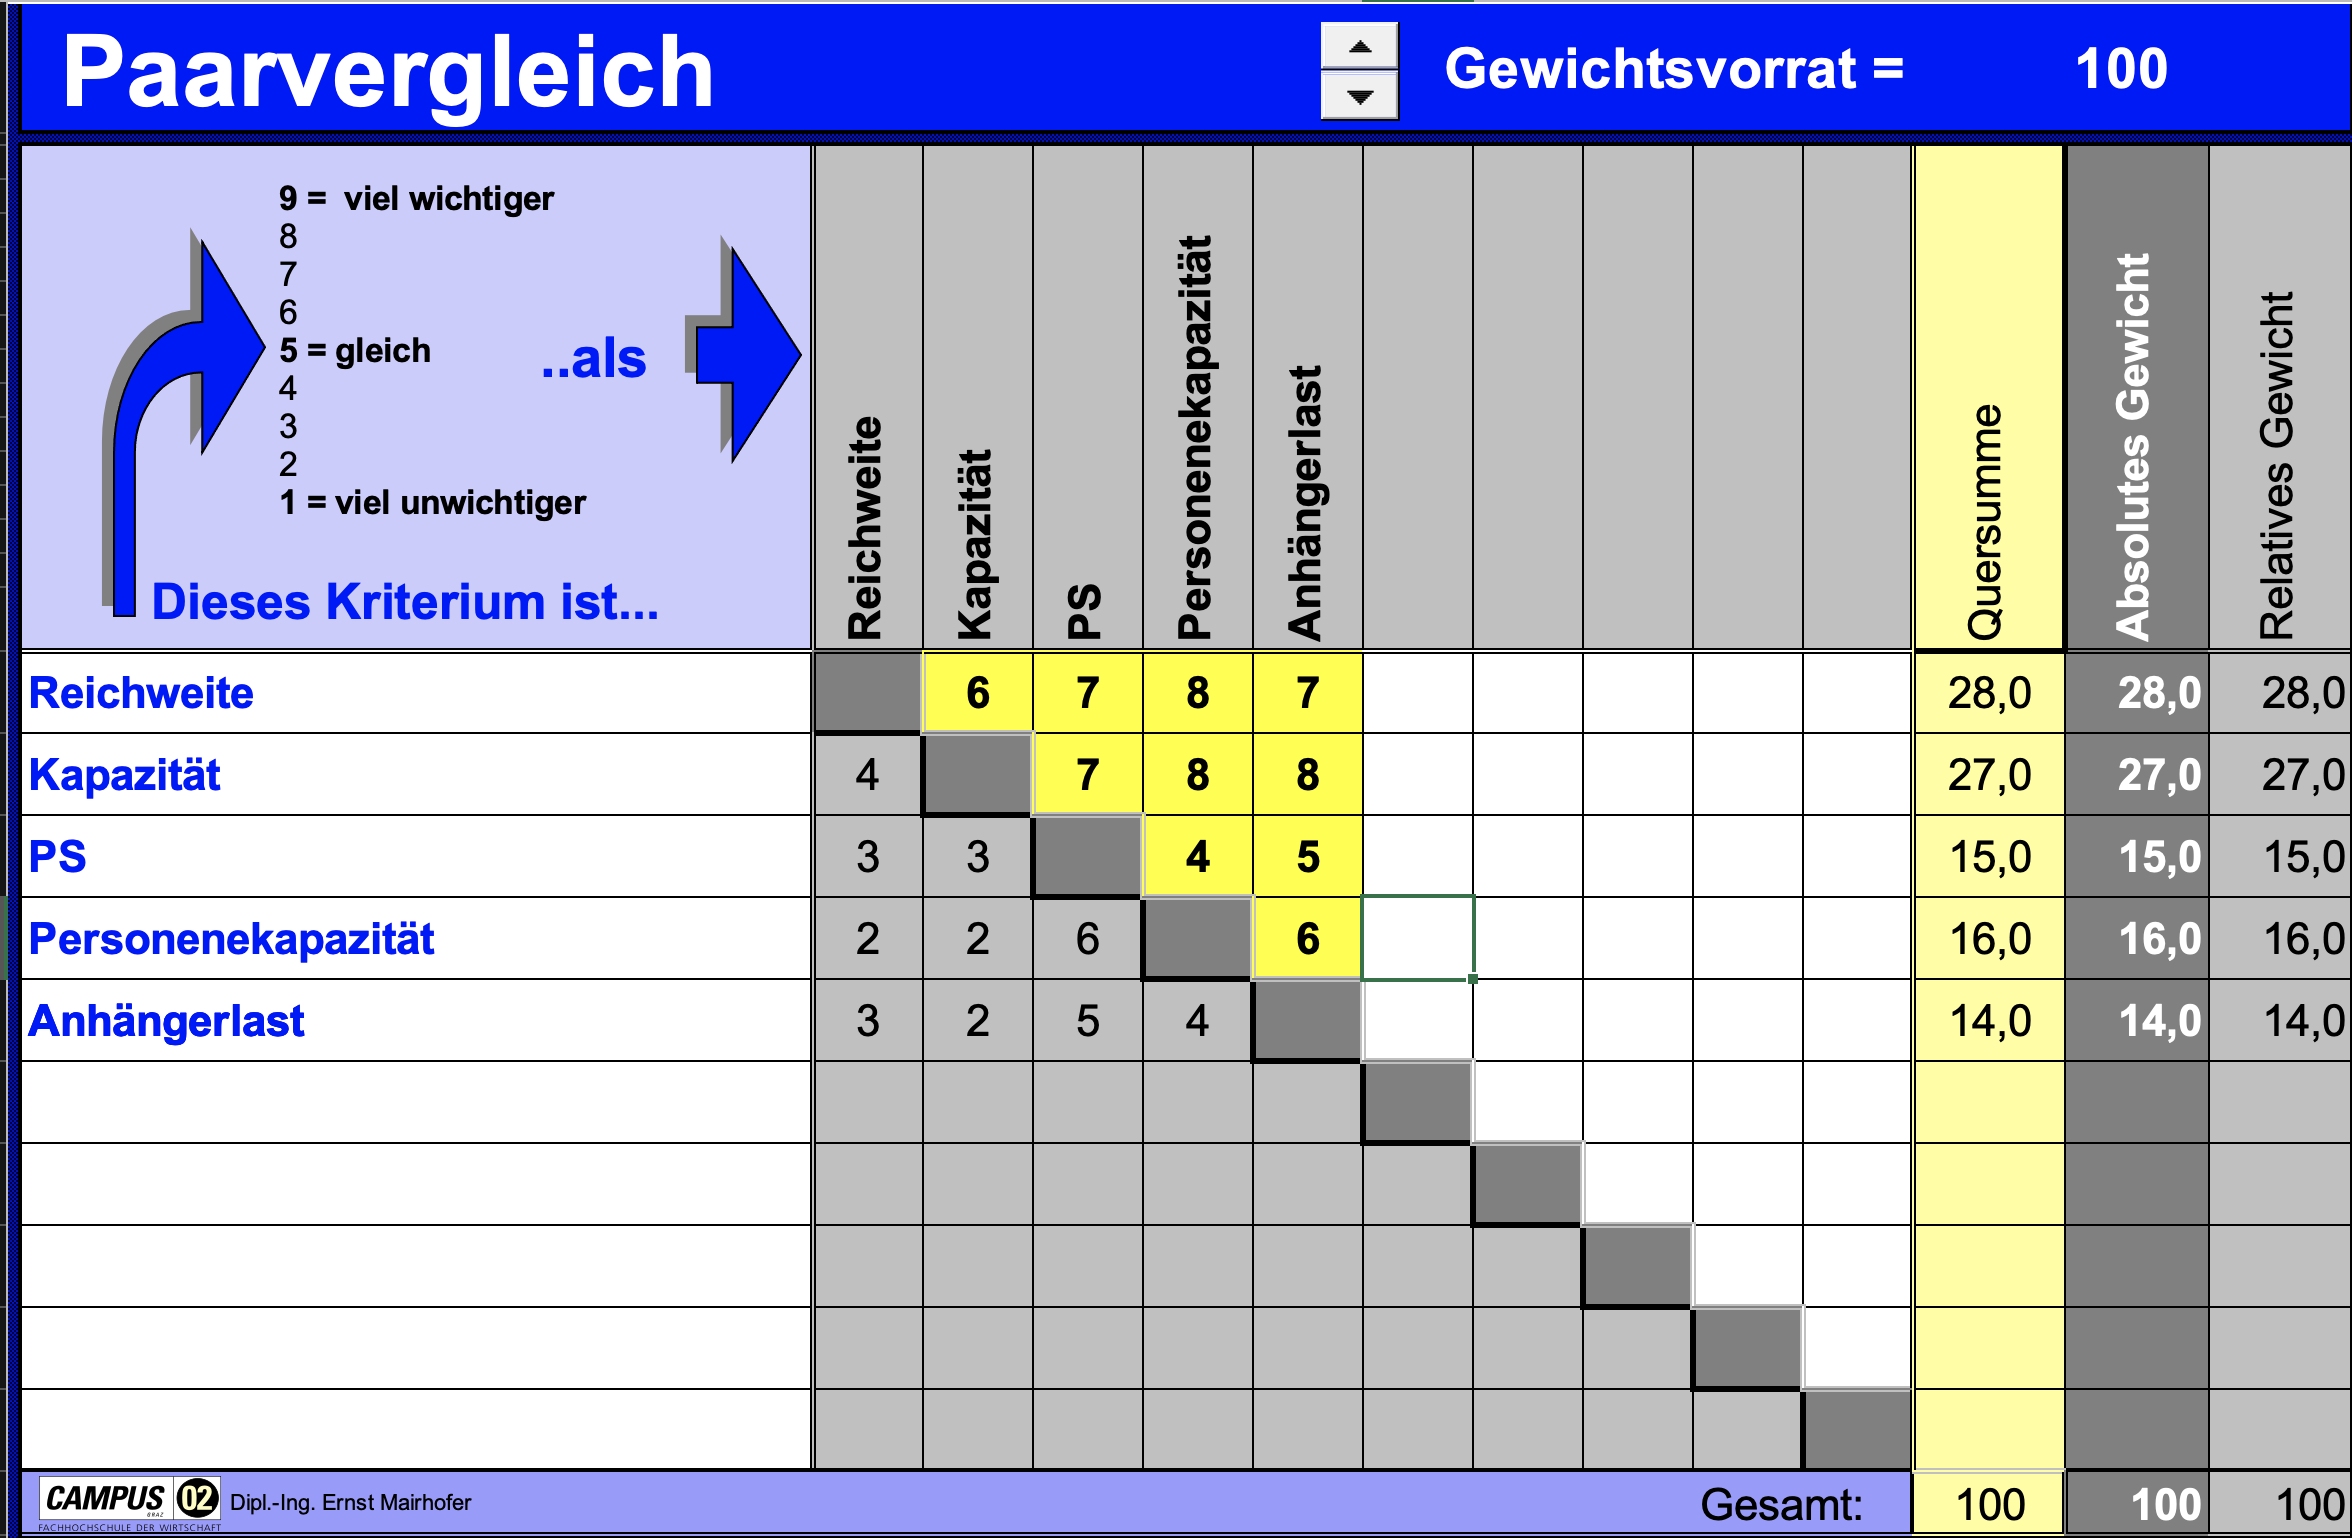
\includegraphics[scale=0.475]{images/paarvergleich.png}
	\caption{Paarvergleich}
	\end{figure}
	\subsection{Entscheidung}
	Preis - 
		Ford - 40.000€
		Iveco - 43.000€
		BYD - 35.000€
	Reichweite
		Ford - 400 km
		Iveco - 400 km
		BYD - 240 km
	Kapazität
	- Nutzlast
	- Nutzraum
	KW
		Ford - 77 kW
		Iveco - 
		BYD - 100 kW
	Personenkapazität
	\section{Projektmanagement}
	\subsection{Abgrenzung Projekt}
	\subsection{Projektabgrenzung und Kontextanalyse}
	\subsection{Leistungsplanung}
	\subsection{Terminplanung}
	\subsection{Ressourcen/Kostenplanung inkl. Risikoanalyse}
	























  
\end{document}